\documentclass[11pt]{article}

\usepackage[margin=1in]{geometry}
\usepackage{amsmath,amssymb,amsthm,mathtools}
\usepackage{graphicx}
\usepackage[hidelinks]{hyperref}

\newtheorem{theorem}{Theorem}
\newtheorem{lemma}{Lemma}
\newtheorem{remark}{Remark}

\newcommand{\N}{\mathbb N}
\newcommand{\C}{\mathbb C}
\newcommand{\B}{\mathcal B}
\newcommand{\ellTwo}{\ell^2}
\newcommand{\norm}[1]{\left\lVert #1\right\rVert}

\title{A Continuous Schur Multiplier with No Continuous Hilbert Factorization}
\author{Automated Math Discovery Candidate Counterexample}
\date{July 22, 2026}

\begin{document}
\maketitle

\begin{center}
\fbox{\parbox{0.91\textwidth}{\textbf{Status.}
Candidate full counterexample, likely valid pending expert review.  It gives a
negative answer to Steen--Todorov--Turowska Question 4.13(i), as predicted in
the target paper.}}
\end{center}

\section*{Source Question}

Steen, Todorov, and Turowska ask in Question 4.13(i) of
\cite{SteenTodorovTurowska} whether every continuous Schur multiplier
$\varphi:X\times X\to\C$ on a locally compact space with a regular Borel
measure has a representation
\[
                 \varphi(x,y)=\langle a(x),b(y)\rangle_{\ellTwo}
\]
with continuous bounded functions $a,b:X\to\ellTwo$.  Arhancet
\cite{Arhancet} proves the positive-kernel version and writes that the answer
to part (i) should be negative.  The example below proves that prediction,
even for a compact metric space with a full-support probability measure.

\begin{center}
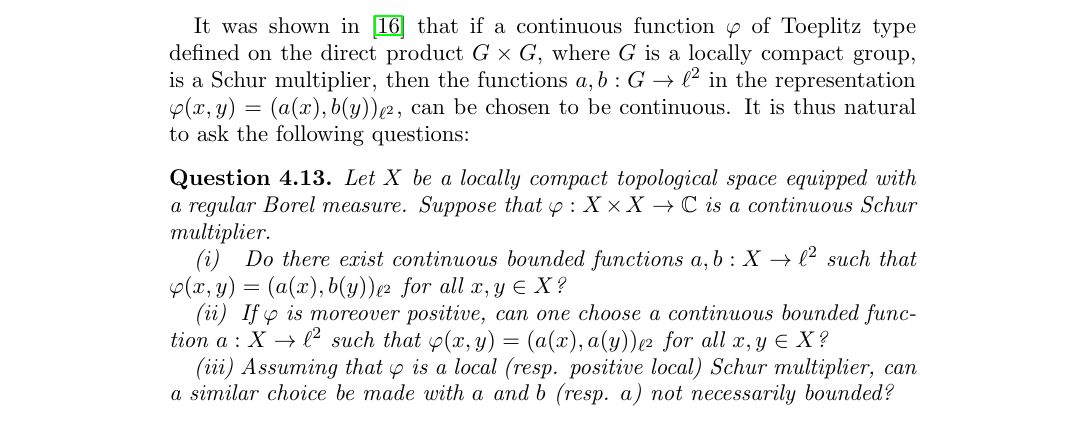
\includegraphics[width=\textwidth]{figures/question_4_13_crop.png}
\end{center}

\section*{Proof Intuition}

Take infinitely many finite Schur multipliers, each of norm one, but make
their scalar entries tend uniformly to zero.  The resulting block diagonal
kernel is continuous after all blocks are joined at one point at infinity.
If continuous Hilbert-space factors existed, subtracting their values at
infinity would make both factors uniformly small on late blocks.  Their
product would then force the Schur multiplier norms of those blocks to tend
to zero, contradicting the norm-one construction.

Normalized Hadamard matrices achieve the needed separation: their entries
are $n^{-1/2}$, while their Schur multiplier norms are exactly one.

\section*{Main Result}

\begin{theorem}\label{thm:main}
There exist a compact metrizable space $X$, a regular Borel probability
measure $\mu$ with full support on $X$, and a continuous function
$\varphi:X\times X\to\C$ such that:
\begin{enumerate}
\item $\varphi$ induces a Schur multiplier
\[
 M_\varphi:\B(L^2(X,\mu))\longrightarrow\B(L^2(X,\mu))
\]
of norm one;
\item there are no continuous functions $a,b:X\to\ellTwo$ satisfying
\[
             \varphi(x,y)=\langle a(x),b(y)\rangle
             \qquad (x,y\in X).
\]
\end{enumerate}
In particular, Question 4.13(i) of \cite{SteenTodorovTurowska} has a negative
answer.  Since $X$ is compact, the word ``bounded'' in that question is
automatic for continuous $a$ and $b$.
\end{theorem}

We first record the elementary factorization estimate that drives the
obstruction.

\begin{lemma}[Factorization bound]\label{lem:factorization}
Let $E$ be a finite set and let $\psi=(\psi_{ij})_{i,j\in E}$.  If
$\psi_{ij}=\langle \xi_i,\eta_j\rangle$ for vectors in a Hilbert space, then
the Schur multiplier $S_\psi$ on $\B(\ell^2(E))$ satisfies
\[
       \norm{S_\psi}\leq
       \left(\sup_{i\in E}\norm{\xi_i}\right)
       \left(\sup_{j\in E}\norm{\eta_j}\right).
\]
\end{lemma}

\begin{proof}
Define $Ue_i=e_i\otimes\xi_i$ and $Ve_j=e_j\otimes\eta_j$.  Up to the
irrelevant choice of inner-product convention,
\[
                       S_\psi(T)=U^*(T\otimes I)V.
\]
Hence $\norm{S_\psi}\leq\norm U\norm V$, which is the displayed bound.
\end{proof}

\begin{proof}[Proof of Theorem \ref{thm:main}]
Let
\[
                         X=\N\cup\{\infty\}
\]
be the one-point compactification of the discrete natural numbers.  Thus
$n\to\infty$ in $X$ as $n\to\infty$ in the usual sense, and $X$ is
homeomorphic to $\{0\}\cup\{1/n:n\geq1\}$.  Put
\[
          \mu(\{n\})=2^{-n}\quad(n\geq1),
          \qquad \mu(\{\infty\})=0.
\]
This is a regular Borel probability measure.  It has full support: every
finite point is a positive-mass open atom, and every neighborhood of
$\infty$ contains a cofinite tail of positive mass.

Partition $\N$ into successive intervals
\[
              I_k=\{2^k-1,2^k,\ldots,2^{k+1}-2\},
              \qquad |I_k|=n_k:=2^k,
              \qquad k\geq1.
\]
Let $H_k$ be the Sylvester Hadamard matrix of order $n_k$.  Thus all its
entries are $\pm1$ and
\[
                         H_kH_k^*=n_kI_{n_k}.
\]
After identifying the rows and columns with $I_k$, define
\begin{equation}\label{eq:kernel}
 \varphi(i,j)=
 \begin{cases}
  n_k^{-1/2}(H_k)_{ij},&i,j\in I_k\text{ for the same }k,\\
  0,&\text{otherwise},
 \end{cases}
 \qquad
 \varphi(\infty,x)=\varphi(x,\infty)=0.
\end{equation}

We check continuity.  Finite points are isolated.  At $(\infty,j)$, where
$j$ is finite, the kernel is identically zero once the first coordinate is
outside the one finite block containing $j$; similarly at $(i,\infty)$.  At
$(\infty,\infty)$, points in distinct blocks give zero, while points in a
common block $I_k$ have absolute value $n_k^{-1/2}=2^{-k/2}\to0$.  This is
exactly the required continuity.

Next we compute the Schur norm.  In the Hilbert direct sum
$\mathcal H=\bigoplus_{k\geq1}\ell^2(I_k)$, let $\xi_i$ be the row of
$n_k^{-1/2}H_k$ corresponding to $i\in I_k$, placed in the $k$th summand,
and let $\eta_j$ be the standard basis vector corresponding to $j\in I_k$
in that same summand.  Then
\[
       \norm{\xi_i}=\norm{\eta_j}=1,
       \qquad \varphi(i,j)=\langle\xi_i,\eta_j\rangle.
\]
The same operator factorization as in Lemma \ref{lem:factorization} gives
$\norm{M_\varphi}\leq1$.  This applies on $L^2(X,\mu)$ because the normalized
atom indicators identify it unitarily with $\ell^2(\N)$, and multiplication
of integral kernels by $\varphi$ becomes entrywise matrix multiplication;
the atom weights cancel in this normalized basis.

The reverse inequality is already visible on every block.  Write
$\varphi_k=n_k^{-1/2}H_k$.  Entrywise multiplication gives
\[
                   S_{\varphi_k}(H_k)
                  =n_k^{-1/2}J_{n_k},
\]
where $J_{n_k}$ is the all-ones matrix.  Since
\[
       \norm{H_k}=\sqrt{n_k},
       \qquad
       \norm{n_k^{-1/2}J_{n_k}}=\sqrt{n_k},
\]
we get $\norm{S_{\varphi_k}}\geq1$.  Compression to the block gives
$\norm{M_\varphi}\geq1$, and hence $\norm{M_\varphi}=1$.

Suppose, toward a contradiction, that continuous $a,b:X\to\ellTwo$ satisfy
$\varphi(x,y)=\langle a(x),b(y)\rangle$ everywhere.  Set
\[
        \widetilde a(x)=a(x)-a(\infty),
        \qquad
        \widetilde b(y)=b(y)-b(\infty).
\]
The three identities
\[
 \langle a(\infty),b(y)\rangle=\varphi(\infty,y)=0,
 \quad
 \langle a(x),b(\infty)\rangle=\varphi(x,\infty)=0,
 \quad
 \langle a(\infty),b(\infty)\rangle=0
\]
show that the centered maps still factor the same kernel:
\[
                 \varphi(x,y)
                 =\langle\widetilde a(x),\widetilde b(y)\rangle.
\]
Continuity at $\infty$ now implies
\[
 A_k:=\sup_{i\in I_k}\norm{\widetilde a(i)}\longrightarrow0,
 \qquad
 B_k:=\sup_{j\in I_k}\norm{\widetilde b(j)}\longrightarrow0.
\]
Applying Lemma \ref{lem:factorization} to the restriction to $I_k\times I_k$
would give
\[
                         1=\norm{S_{\varphi_k}}
                         \leq A_kB_k\longrightarrow0,
\]
an impossibility.  Thus no continuous Hilbert factorization exists.
\end{proof}

\section*{Scope and Novelty}

The counterexample is not positive; this is necessary because the positive
case was proved affirmatively in \cite{Arhancet}.  It uses only a compact
convergent sequence, a full-support probability measure, and real-valued
kernels.  Bounded searches through July 22, 2026 found the original question,
Arhancet's negative prediction, and general factorization literature, but no
published counterexample of this form.  Novelty confidence is therefore
moderate pending a specialist literature review.

\begin{thebibliography}{9}

\bibitem{Arhancet}
C.~Arhancet,
\emph{Dilations of Markovian semigroups of measurable Schur multipliers},
Canad. J. Math. 74 (2022), 59--93; arXiv:1910.14434.

\bibitem{SteenTodorovTurowska}
N.~M. Steen, I.~G. Todorov, and L.~Turowska,
\emph{Local operator multipliers and positivity},
J. Funct. Anal. 267 (2014), 80--111; arXiv:1206.3889.

\end{thebibliography}

\end{document}
